\section{Introduction}
\label{sec:introduction}

% \section*{Intro guidance}

Just to clarify the goal of this project is to use kinematic maps to ascertain if the post-starburst galaxies are caused by mergers (i.e. post-mergers). 

There are another couple of papers to look at:
Stark et al. 2018: \citep{2018MNRAS.480.2217S} 
Barrera-Ballesteros et al. 2015: \citep{2015A&A...582A..21B}
 
Once you have looked at these, could you move up and down the references and cited papers in each paper, and see if you can find any other methods that have been used to identify merger or post-merger features \textbf{using kinematic features or maps}?
 
Extend your report to perhaps 1.5-2 pages to give a complete summary of the literature.

On discussion with Anne-Marie, we are not convinced that the full kinemetry fits will provide useful data on MaNGA galaxies. Note that it is important to get good marks on your final report that you provide a critical assessment of both your results and previous results, so have a think about the methods and what might work / not work on the MaNGA galaxies. 

\vspace{6pt}
\textbf{Remember to remove redundant subsection outlining placeholders.}


\subsection{Post starburst Galaxies}
[TODO: write a piece on PSBs and their significance in the theory of galaxy evolution.] Include a piece on the SDSS MaNGA survey employed in the science.

Vivienne has been involved in the preparation of a number of papers researching PSBs: \citet{2017MNRAS.472.1401A} regarding the relationship between quenching of star formation and morphological transition, while \citet{2016MNRAS.463..832W} sets out the background work.
[TODO: write a piece on PSBs and their significance in the theory of galaxy evolution.]

\subsection{Galaxy evolution}
\label{sec:evolution}

The prevalent theory of galaxy evolution is often explained  by  by referring to galaxy colour-colour and colour-magnitude diagrams (CMD) \citep[see e.g.][]{2001AJ....122.1861S, 2003ApJ...585L...5H, 2003ApJS..149..289B,baldry2004quantifying,2006MNRAS.373..469B}. A representative CMD constructed from SDSS observations of 20,000 nearby galaxies is presented in  Figure~\ref{fig:CMD1}. Gas-rich, star-forming, often disc-like galaxies populate the so-called 'blue cloud' region of the CMD. As gas is consumed through star formation blue cloud galaxies are understood to transition to the redder mainly early-type elliptical quiescent galaxies along the upper left in the 'red sequence' region of the CMD. There is a sparsely populated region separating the blue cloud and red sequence populations often referred to as the 'green valley' region of the CMD  \citep{2004ApJ...608..752B}. In this paper we explore the evolutionary pathway of galaxies in transition between the blue cloud and the red sequence, through the green valley.
It is of interest to note \citet{Mutch_2011} claim that the Milky Way and the Andromeda galaxy M31 are in evolutionary transition due to consumption of cold gas and both lie within the green valley region of the galaxy CMD.

\begin{figure}
	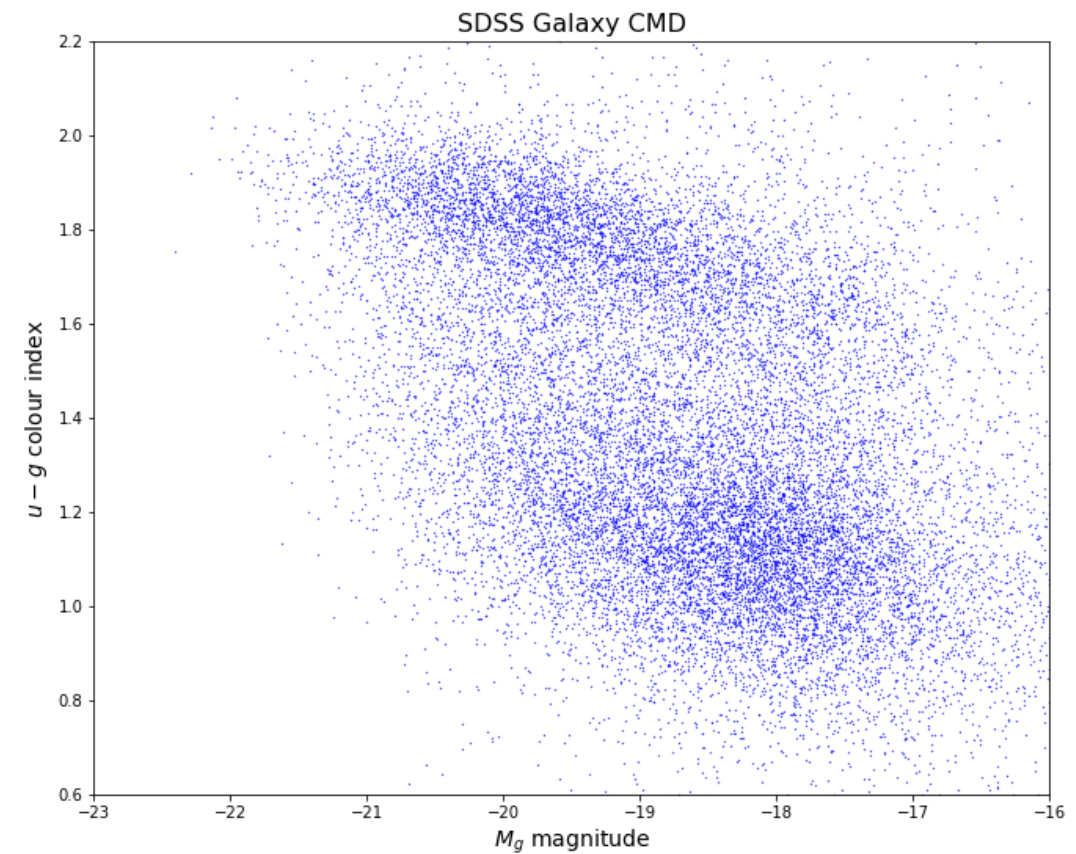
\includegraphics[width=\columnwidth]{images/CMDs/galaxyCMD.PNG}
    \caption{Galaxy colour-magnitude diagram: $u-g$ colour index versus $M_g$ magnitude. The bimodality of the distribution is discussed in the text.}
    \label{fig:CMD1}
\end{figure}

\subsection{SDSS IV MaNGA}
An overview of the SDSS MaNGA project is provided by \citet{2015ApJ...798....7B}. A concise description of the \href{https://iopscience.iop.org/article/10.1088/0004-637X/798/1/7/meta#apj504473s3}{survey design} is included in Section 3. We use data release DR15 of the SDSS MaNGA-IV survey \citep{2019ApJS..240...23A} and the associated FITS-format galaxy data summary table output from the MaNGA data reduction pipeline (DRP) \texttt{drpall} file version 2.4.3 as described by \citet{2016AJ....152...83L}. The output of the DRP is fed to the MaNGA data analysis pipeline (DAP) which, for DR15 and the purposes of this paper provides:
\begin{itemize}
    \item Spatially stacked spectra
    \item Stellar kinematics (V and $\sigma$)
    \item Nebular emission-line properties: fluxes, equivalent widths, and kinematics (V and $\sigma$)
    \item Spectral Indices: absorption-line (e.g., H$\delta)$ and bandhead (e.g., D4000) measurements
\end{itemize}

DRP fields of interest used in this project are listed in Table \ref{tab:DRPall-table}.

\begin{table*}
\caption[MaNGA DRPALL fields]{SDSS MaNGA DPPRALL data fields of interest}
\label{tab:DRPall-table}
\begin{tabular}{|p{3.2cm}|p{1.2cm}||p{1cm}|p{10cm}|}
\hline
Name & Type & Unit & Description \\
\hline
PLATEIFU & char{[}100{]} &  & Plate+ifudesign name for this object (e.g. 7443-12701)\\
MANGAID & char{[}100{]} & & MaNGA ID for this object (e.g. 1-114145)\\
OBJRA & float64 & degrees & Right ascension of the science object in J2000\\
OBJDEC & float64 & degrees & Declination of the science object in J2000\\
NSA\_Z & float64 &  & Heliocentric redshift\\
NSA\_ZDIST & float64 &  & Distance estimate using peculiar velocity model of Willick et al. (1997); mulitply by c/Ho for Mpc\\
NSA\_ELPETRO\_MASS & float64 &  & Stellar mass from K-correction fit (use with caution) for elliptical Petrosian fluxes (Ωm=0.3, ΩΛ=0.7, h=1)\\
NSA\_ELPETRO\_BA & float64 &  & Axis ratio used for elliptical apertures (for this version, same as ba90)\\
NSA\_ELPETRO\_TH50\_R & float64 & arcsec & Elliptical Petrosian 50\% light radius in SDSS r-band\\
NSA\_SERSIC\_N & float64 &  & Se
rsic index from two-dimensional, single-component Sersic fit in r-band\\
\hline
\end{tabular}
\end{table*}

\subsection{Structure of the paper}
The content of the paper is organised as follows: A concise review of the literature on galaxy mergers and morphology transitions relevant to the paper is introduced in Section \ref{sec:mergers}. The selection criteria for the PSB sample and control galaxies are laid out in Section \ref{sec:sample}. Data analysis methods and results are presented in Section \ref{sec:analysis}. The method of the velocity field analysis method employing the Radon transform method is a significant analysis tool in its own right. This is discussed in some detail in Section \ref{sec:Radon}. Finally, a summary of the research and the conclusions drawn from this work, along with recommendations for further study are presented in Section \ref{sec:discussion}.
